% Created by tikzDevice version 0.11 on 2018-03-18 23:48:13
% !TEX encoding = UTF-8 Unicode
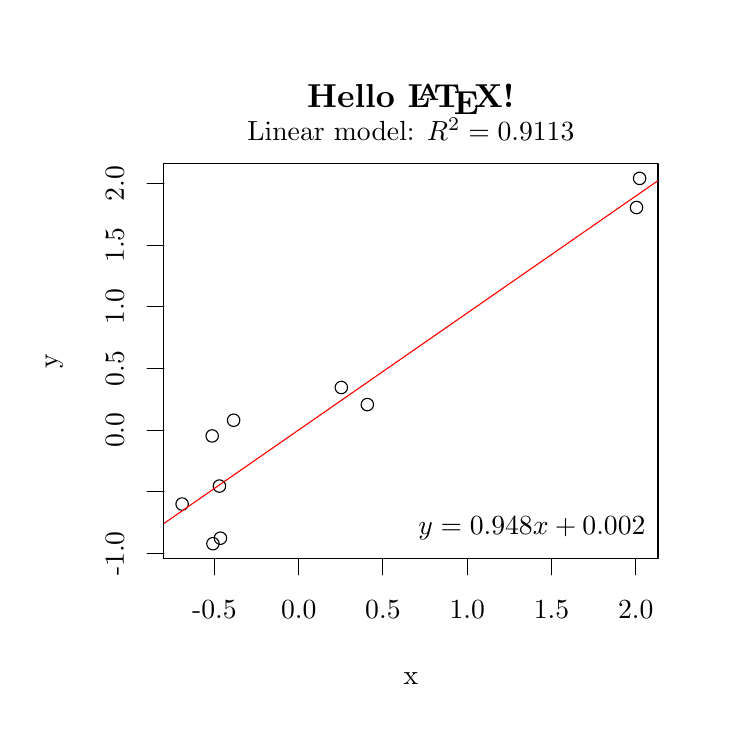
\begin{tikzpicture}[x=1pt,y=1pt]
\definecolor{fillColor}{RGB}{255,255,255}
\path[use as bounding box,fill=fillColor,fill opacity=0.00] (0,0) rectangle (252.94,252.94);
\begin{scope}
\path[clip] ( 49.20, 61.20) rectangle (227.75,203.75);
\definecolor{drawColor}{RGB}{0,0,0}

\path[draw=drawColor,line width= 0.4pt,line join=round,line cap=round] ( 74.42,111.08) circle (  2.25);

\path[draw=drawColor,line width= 0.4pt,line join=round,line cap=round] ( 69.29, 87.30) circle (  2.25);

\path[draw=drawColor,line width= 0.4pt,line join=round,line cap=round] (122.73,116.74) circle (  2.25);

\path[draw=drawColor,line width= 0.4pt,line join=round,line cap=round] (113.33,122.92) circle (  2.25);

\path[draw=drawColor,line width= 0.4pt,line join=round,line cap=round] ( 66.94, 66.48) circle (  2.25);

\path[draw=drawColor,line width= 0.4pt,line join=round,line cap=round] ( 66.67,105.41) circle (  2.25);

\path[draw=drawColor,line width= 0.4pt,line join=round,line cap=round] (221.13,198.47) circle (  2.25);

\path[draw=drawColor,line width= 0.4pt,line join=round,line cap=round] (220.00,187.95) circle (  2.25);

\path[draw=drawColor,line width= 0.4pt,line join=round,line cap=round] ( 55.81, 80.81) circle (  2.25);

\path[draw=drawColor,line width= 0.4pt,line join=round,line cap=round] ( 69.66, 68.47) circle (  2.25);
\end{scope}
\begin{scope}
\path[clip] (  0.00,  0.00) rectangle (252.94,252.94);
\definecolor{drawColor}{RGB}{0,0,0}

\path[draw=drawColor,line width= 0.4pt,line join=round,line cap=round] ( 67.48, 61.20) -- (219.72, 61.20);

\path[draw=drawColor,line width= 0.4pt,line join=round,line cap=round] ( 67.48, 61.20) -- ( 67.48, 55.20);

\path[draw=drawColor,line width= 0.4pt,line join=round,line cap=round] ( 97.93, 61.20) -- ( 97.93, 55.20);

\path[draw=drawColor,line width= 0.4pt,line join=round,line cap=round] (128.37, 61.20) -- (128.37, 55.20);

\path[draw=drawColor,line width= 0.4pt,line join=round,line cap=round] (158.82, 61.20) -- (158.82, 55.20);

\path[draw=drawColor,line width= 0.4pt,line join=round,line cap=round] (189.27, 61.20) -- (189.27, 55.20);

\path[draw=drawColor,line width= 0.4pt,line join=round,line cap=round] (219.72, 61.20) -- (219.72, 55.20);

\node[text=drawColor,anchor=base,inner sep=0pt, outer sep=0pt, scale=  1.00] at ( 67.48, 39.60) {-0.5};

\node[text=drawColor,anchor=base,inner sep=0pt, outer sep=0pt, scale=  1.00] at ( 97.93, 39.60) {0.0};

\node[text=drawColor,anchor=base,inner sep=0pt, outer sep=0pt, scale=  1.00] at (128.37, 39.60) {0.5};

\node[text=drawColor,anchor=base,inner sep=0pt, outer sep=0pt, scale=  1.00] at (158.82, 39.60) {1.0};

\node[text=drawColor,anchor=base,inner sep=0pt, outer sep=0pt, scale=  1.00] at (189.27, 39.60) {1.5};

\node[text=drawColor,anchor=base,inner sep=0pt, outer sep=0pt, scale=  1.00] at (219.72, 39.60) {2.0};

\path[draw=drawColor,line width= 0.4pt,line join=round,line cap=round] ( 49.20, 62.92) -- ( 49.20,196.67);

\path[draw=drawColor,line width= 0.4pt,line join=round,line cap=round] ( 49.20, 62.92) -- ( 43.20, 62.92);

\path[draw=drawColor,line width= 0.4pt,line join=round,line cap=round] ( 49.20, 85.21) -- ( 43.20, 85.21);

\path[draw=drawColor,line width= 0.4pt,line join=round,line cap=round] ( 49.20,107.50) -- ( 43.20,107.50);

\path[draw=drawColor,line width= 0.4pt,line join=round,line cap=round] ( 49.20,129.79) -- ( 43.20,129.79);

\path[draw=drawColor,line width= 0.4pt,line join=round,line cap=round] ( 49.20,152.09) -- ( 43.20,152.09);

\path[draw=drawColor,line width= 0.4pt,line join=round,line cap=round] ( 49.20,174.38) -- ( 43.20,174.38);

\path[draw=drawColor,line width= 0.4pt,line join=round,line cap=round] ( 49.20,196.67) -- ( 43.20,196.67);

\node[text=drawColor,rotate= 90.00,anchor=base,inner sep=0pt, outer sep=0pt, scale=  1.00] at ( 34.80, 62.92) {-1.0};

\node[text=drawColor,rotate= 90.00,anchor=base,inner sep=0pt, outer sep=0pt, scale=  1.00] at ( 34.80,107.50) {0.0};

\node[text=drawColor,rotate= 90.00,anchor=base,inner sep=0pt, outer sep=0pt, scale=  1.00] at ( 34.80,129.79) {0.5};

\node[text=drawColor,rotate= 90.00,anchor=base,inner sep=0pt, outer sep=0pt, scale=  1.00] at ( 34.80,152.09) {1.0};

\node[text=drawColor,rotate= 90.00,anchor=base,inner sep=0pt, outer sep=0pt, scale=  1.00] at ( 34.80,174.38) {1.5};

\node[text=drawColor,rotate= 90.00,anchor=base,inner sep=0pt, outer sep=0pt, scale=  1.00] at ( 34.80,196.67) {2.0};

\path[draw=drawColor,line width= 0.4pt,line join=round,line cap=round] ( 49.20, 61.20) --
	(227.75, 61.20) --
	(227.75,203.75) --
	( 49.20,203.75) --
	( 49.20, 61.20);
\end{scope}
\begin{scope}
\path[clip] (  0.00,  0.00) rectangle (252.94,252.94);
\definecolor{drawColor}{RGB}{0,0,0}

\node[text=drawColor,anchor=base,inner sep=0pt, outer sep=0pt, scale=  1.20] at (138.47,224.20) {\bfseries Hello \LaTeX!};

\node[text=drawColor,anchor=base,inner sep=0pt, outer sep=0pt, scale=  1.00] at (138.47, 15.60) {x};

\node[text=drawColor,rotate= 90.00,anchor=base,inner sep=0pt, outer sep=0pt, scale=  1.00] at ( 10.80,132.47) {y};
\end{scope}
\begin{scope}
\path[clip] ( 49.20, 61.20) rectangle (227.75,203.75);
\definecolor{drawColor}{RGB}{255,0,0}

\path[draw=drawColor,line width= 0.4pt,line join=round,line cap=round] ( 49.20, 73.76) -- (227.75,197.65);
\end{scope}
\begin{scope}
\path[clip] (  0.00,  0.00) rectangle (252.94,252.94);
\definecolor{drawColor}{RGB}{0,0,0}

\node[text=drawColor,anchor=base,inner sep=0pt, outer sep=0pt, scale=  1.00] at (138.47,212.14) {Linear model: $R^{2}= 0.9113 $};
\end{scope}
\begin{scope}
\path[clip] ( 49.20, 61.20) rectangle (227.75,203.75);
\definecolor{drawColor}{RGB}{0,0,0}

\node[text=drawColor,anchor=base west,inner sep=0pt, outer sep=0pt, scale=  1.00] at (141.16, 69.76) {$y = 0.948x +0.002$};
\end{scope}
\end{tikzpicture}
